%% -*- coding: utf-8 -*-
\documentclass[12pt,a4paper]{scrartcl} 
\usepackage[utf8]{inputenc}
\usepackage[english,russian]{babel}
\usepackage{indentfirst}
\usepackage{misccorr}
\usepackage{graphicx}
\usepackage{amsmath}
\begin{document}

\section{Текстовая формулировка задачи}
\label{sec:exp}
 \ {Цель работы: Построение массива методом быстрой сортировки и методом слияния}




\section{Ход работы}
\label{sec:exp}

\subsection{Код приложения}
\label{sec:exp:code}
\begin{verbatim}
   #include <stdio.h>
#include <stdlib.h>
#include <iostream>
using namespace std;
void quickSort(int a[], int l, int r)
{
    setlocale(LC_ALL, "RUSSIAN");
    int i = l;
    int j = r;
    int sred = a[(l + r) / 2];
    do {
        while (a[i] < sred) i++;
        while (a[j] > sred) j--;
        if (i <= j)
        {
            int w = a[i];
            a[i] = a[j];
            a[j] = w;
            i++;
            j--;
        }
    } while (i < j);
    if (l < j) quickSort(a, l, j);
    if (r < i) quickSort(a, i, r);
}
void merge(int a[], int l, int r, int sred);
 
void mergeSort(int a[], int l, int r)
{
    int sred;
    if (l < r) {
 
        sred = (l + r) / 2;
        mergeSort(a, l, sred);
        mergeSort(a, sred + 1, r);
        merge(a, l, r, sred);
    }
}
void merge(int a[], int l, int r, int sred)
{
    int a1[8];
    int i, j, k;
    i = l;
    k = l;
    j = sred + 1;
 
    while (i <= sred && j <= r) {
        if (a[i] < a[j]) {
            a1[k] = a[i];
            k++;
            i++;
        }
        else {
            a1[k] = a[j];
            k++;
            j++;
        }
    }
 
    while (i <= sred) {
        a1[k] = a[i];
        k++;
        i++;
    }
 
    while (j <= r) {
        a1[k] = a[j];
       k++;
        j++;
   }
 
    for (i = l; i < k; i++) {
        a[i] = a1[i];
    }
}
 
int main()
{
    setlocale(LC_ALL, "Rus");
    int i = 0;
 
    const int n = 5;
    int a[n];
    cout << "Введите цифры" << endl;
    for (int i = 0; i < n; i++)
    {
        cin >> a[i];
    }
    cout << "Исходный массив" << endl;
    for (int i = 0; i < n; i++)
    {
        cout << a[i] << " ";
    }
    cout << endl;
    int v;
    cout << " Метод сортировки :" << endl << "1 ) Быстрая сортировка" << endl << "2 ) Сортировка слиянием" << endl;
    cin >> v;
    if (v == 1) {
        quickSort(a, i, n);
    }
   else if (v == 2) {
        mergeSort(a, i, n);
    }
    else {
        return 0;
    }
    {
    cout << "Массив после сортировки" << endl;
    for (int i = 0; i < n; i++)
    {
        cout << a[i] << " ";
    }
    return 0;
} 
}
\end{verbatim}

\section{Скриншот программы}
\label{sec:intro}
\centering
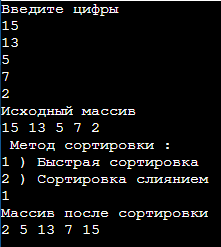
\includegraphics[scale=1.32]{var1.png}
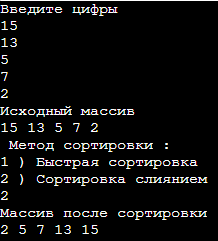
\includegraphics[scale=1.35]{var2.png}
\caption{1. Результат программы.}\label{fig:par}
\section{Пример библиографических ссылок}

Для изучения «внутренностей» \TeX{} необходимо 
изучить~\cite{Knuth-2003}, а для использования \LaTeX{} лучше
почитать~\cite{Lvovsky-2003, Voroncov-2005}.

\begin{thebibliography}{9}
\bibitem{Knuth-2003}Кнут Д.Э. Всё про \TeX. \newblock --- Москва: Изд. Вильямс, 2003 г. 550~с.
\bibitem{Lvovsky-2003}Львовский С.М. Набор и верстка в системе \LaTeX{}. \newblock --- 3-е издание, исправленное и дополненное, 2003 г.
\bibitem{Voroncov-2005}Воронцов К.В. \LaTeX{} в примерах. 2005 г.
\end{thebibliography}

\end{document}
